% ============================================================
% IskolE – Second Year Group Project Report
% CS Group 38 | SCS2202 – Group Project
% ============================================================
\documentclass[12pt, a4paper]{report}

% ── Packages ─────────────────────────────────────────────────
\usepackage[utf8]{inputenc}
\usepackage[T1]{fontenc}
\usepackage{lmodern}
\usepackage[margin=2.5cm]{geometry}
\usepackage{graphicx}
\usepackage{booktabs}
\usepackage{longtable}
\usepackage{enumitem}
\usepackage{hyperref}
\usepackage{xcolor}
\usepackage{titlesec}
\usepackage{fancyhdr}
\usepackage{setspace}
\usepackage{parskip}
\usepackage{caption}
\usepackage{float}
\usepackage{array}
\usepackage{tabularx}
\usepackage{colortbl}       % For \rowcolor in tables
\usepackage{pgf-pie}       % For the contribution pie chart
\usepackage{tikz}

% ── Light Blue Color Theme ───────────────────────────────────
\definecolor{themeblue}{HTML}{2B7BBF}
\definecolor{themelightblue}{HTML}{D6EAF8}
\definecolor{themedarkblue}{HTML}{1A5276}
\definecolor{themeaccent}{HTML}{3498DB}

% ── Page Style ───────────────────────────────────────────────
\pagestyle{fancy}
\fancyhf{}
\fancyhead[L]{\small\color{themedarkblue} IskolE – School Management System}
\fancyhead[R]{\small\color{themedarkblue} CS Group 38}
\fancyfoot[C]{\thepage}
\renewcommand{\headrulewidth}{0.4pt}
\renewcommand{\footrulewidth}{0pt}

% ── Hyperlink Style ──────────────────────────────────────────
\hypersetup{
    colorlinks=true,
    linkcolor=themedarkblue,
    urlcolor=themeaccent,
    citecolor=themedarkblue
}

% ── Spacing ──────────────────────────────────────────────────
\setstretch{1.5}

% ── Chapter/Section Formatting (Light Blue Theme) ────────────
\titleformat{\chapter}[display]
  {\normalfont\huge\bfseries\color{themeblue}}{\chaptertitlename\ \thechapter}{20pt}{\Huge\color{themedarkblue}}
\titlespacing*{\chapter}{0pt}{-20pt}{30pt}

\titleformat{\section}
  {\normalfont\Large\bfseries\color{themeblue}}{\thesection}{1em}{}
\titleformat{\subsection}
  {\normalfont\large\bfseries\color{themedarkblue}}{\thesubsection}{1em}{}

% ============================================================
\begin{document}

% ────────────────────────────────────────────────────────────
%                     COVER PAGE
% ────────────────────────────────────────────────────────────
\begin{titlepage}
    \centering
    \vspace*{0.2cm}

    {\Huge\textbf{\color{themedarkblue}IskolE}}\\[0.3cm]
    {\LARGE\textbf{\color{themeblue}The School Management System}}\\[0.8cm]

    {\Large\textbf{\color{themedarkblue}SECOND YEAR GROUP PROJECT REPORT}}\\[0.3cm]
    {\large SCS2202 -- Group Project}\\[0.5cm]

    {\Large\textbf{CS Group: 38}}\\[0.5cm]

    {\color{themeblue}\rule{0.8\textwidth}{0.4pt}}\\[0.5cm]

    {\large\textbf{\color{themedarkblue}Group Member Details}}\\[0.3cm]
    \begin{table}[H]
    \centering
    \renewcommand{\arraystretch}{1.5}
    \begin{tabular}{|c|l|}
    \hline
    \rowcolor{themelightblue}
    \textbf{Index Number} & \textbf{Full Name} \\
    \hline
    23001879 & Seniru D S Senaweera \\
    \hline
    23000821 & R K K Jinendra \\
    \hline
    23000104 & R. S. R. G. A. A. Ananda \\
    \hline
    23001542 & S. K. Thasindu Ramsitha \\
    \hline
    \end{tabular}
    \end{table}

    \vspace{0.3cm}
    {\color{themeblue}\rule{0.8\textwidth}{0.4pt}}\\[0.5cm]

    {\large
    \textbf{Project Supervisor:} Mr.\ Viraj Welgama\\[0.2cm]
    \textbf{Project Co-Supervisor:} Mr.\ Janitha Dissanayake
    }\\[0.8cm]

    {\large University of Colombo School of Computing}\\[0.2cm]
    {\large \the\year}

    \vfill
\end{titlepage}

% ────────────────────────────────────────────────────────────
%                   TABLE OF CONTENTS
% ────────────────────────────────────────────────────────────
\tableofcontents
\newpage

% ────────────────────────────────────────────────────────────
%                   LIST OF FIGURES
% ────────────────────────────────────────────────────────────
\listoffigures
\newpage

% ────────────────────────────────────────────────────────────
%                   LIST OF TABLES
% ────────────────────────────────────────────────────────────
\listoftables
\newpage

% ============================================================
%          CHAPTER 1 – INTRODUCTION
% ============================================================
\chapter{Introduction}

IskolE is a web-based School Management System (SMS) designed to streamline academic, administrative, and communication workflows for Sri Lankan schools. It centralises core activities such as marks/grade management, attendance \& leave, timetabling, announcements, learning materials, and performance analytics while enforcing role-based access for Administrators, Management, Teachers, Parents, and Students.

This report consolidates the proposal into a complete software engineering document covering feasibility, requirements, architecture (using the MVC pattern), system design, implementation completeness, testing, and individual contributions.

% ── 1.1 Domain Description ──────────────────────────────────
\section{Domain Description}

The domain is school operations: academic record keeping; parent--teacher--student communication; attendance and leave handling; class, exam, and annual academic scheduling; and dissemination of learning materials and announcements. The system's stakeholders interact via a secure web application with role-scoped permissions.

% ── 1.2 Current System and Limitations ──────────────────────
\section{Current System and Limitations}

Many schools still rely on paper logs or ad-hoc spreadsheets and verbal/noticeboard communication. This leads to:
\begin{itemize}
    \item Data entry errors
    \item Poor transparency of performance and attendance
    \item Delayed reporting
    \item Manual compilation overhead for administrators
    \item Fragmented communication channels
\end{itemize}

% ── 1.3 Goals & Objectives ─────────────────────────────────
\section{Goals \& Objectives}

\begin{itemize}
    \item Improve communication via structured announcements and dashboards.
    \item Provide real-time access to marks, ranks, and progress analytics for authorised users.
    \item Centralise documents and learning materials.
    \item Automate timetables and event scheduling with reminders.
    \item Support behaviour/remarks logs and comprehensive student profiles.
    \item Enforce secure, role-based access and privacy.
    \item Reduce administrative overhead through automation and reporting.
\end{itemize}

% ── 1.4 Assumptions ────────────────────────────────────────
\section{Assumptions}

\begin{itemize}
    \item Users have internet access and valid emails.
    \item One role per account; unique email; role-scoped data access.
    \item The school must provide the foundation data, and the system builds everything else on top of it.
\end{itemize}

% ============================================================
%          CHAPTER 2 – FEASIBILITY STUDY
% ============================================================
\chapter{Feasibility Study}

% ── 2.1 Technical Feasibility ──────────────────────────────
\section{Technical Feasibility}

In this section we measure how feasible our solution is in a real-world scenario using selected technologies and methods.

\subsection{Front-End Technologies}
\begin{itemize}
    \item \textbf{HTML, CSS, and JavaScript:} These technologies are used to create a responsive and interactive user interface.
\end{itemize}

\subsection{Back-End Technologies}
\begin{itemize}
    \item \textbf{PHP:} PHP is used for handling server-side logic, managing user sessions, server-side requests, and interacting with the MySQL database.
\end{itemize}

\subsection{Environmental Technologies}
\begin{itemize}
    \item \textbf{Docker:} Docker is used for containerisation and deployment of the application. This allows for easy deployment, scalability, and consistency across development and production environments.
\end{itemize}

\subsection{Database Management}
\begin{itemize}
    \item \textbf{MySQL:} MySQL is used to manage databases; SQL queries execute via PHP from the backend.
\end{itemize}

\subsection{Version Control and Collaboration}
\begin{itemize}
    \item \textbf{Git/GitHub:} The Git version control system and GitHub are used to facilitate collaborative contributions from every group member.
    \item \textbf{Jira:} Jira is used for task management and team collaboration, allowing efficient scheduling and development planning.
\end{itemize}

Most of the technologies mentioned above are freely available or open source. The team gained further knowledge and became more familiar with these technologies during the development phase. The free version of Jira was used for task management and team collaboration.

% ── 2.2 Schedule Feasibility ──────────────────────────────
\section{Schedule Feasibility}

Schedule feasibility focuses on whether the project can be successfully completed within the given timeframe, using the available resources and technologies.

\subsection{Project Timeline}
This project spans a full academic year, with development distributed across the first and second semesters.

\subsection{Deliverables}
An interim presentation was delivered after the first semester examinations, showcasing all finalised and implemented user interfaces of the system. The complete system was developed and finalised for submission after the second semester examinations.

\subsection{Resource Availability}
All team members worked on this project alongside their regular academic responsibilities during both semesters. Time was planned to ensure consistent progress while balancing academic workload.

\subsection{Tools Used for Planning}
Jira was used to schedule tasks, assign responsibilities, and track progress throughout the project lifecycle, helping the team stay on track and meet all major deadlines.

% ── 2.3 Resource Feasibility ──────────────────────────────
\section{Resource Feasibility}

\subsection{Human Resources}
The project team consists of four dedicated members who worked collaboratively throughout the first and second semesters. Each member contributed their time and effort alongside academic responsibilities, ensuring steady progress during the academic year.

\subsection{Technical Resources}
Development and testing were carried out using the team's personal computers, which are adequately equipped for the project's needs.

\subsection{Knowledge and Skills}
The team gained foundational knowledge of relevant technologies during the first year of study and continued to expand understanding and practical skills as the project progressed, ensuring readiness for implementation and deployment phases.

% ── 2.4 Operational Feasibility ───────────────────────────
\section{Operational Feasibility}

Focuses on efficiently managing resources, optimising workflows, mitigating risks, and maintaining accurate documentation to streamline project execution.

\begin{itemize}
    \item \textbf{Resource Allocation:} Efficiently managing resources such as time, budget, and equipment.
    \item \textbf{Workflow Management:} Streamlining processes to maximise productivity.
    \item \textbf{Risk Management:} Identifying and reducing risks that could impact project success.
    \item \textbf{Documentation and Reporting:} Ensuring accurate and timely documentation of project progress and outcomes.
\end{itemize}

% ── 2.5 Economic Feasibility ──────────────────────────────
\section{Economic Feasibility}

Manages project costs within budget constraints, ensures financial sustainability and return on investment, and conducts cost-benefit analyses to justify project expenditures.

\begin{itemize}
    \item \textbf{Cost Management:} Controlling project expenses within planned budgets.
    \item \textbf{Financial Sustainability:} Ensuring long-term financial viability and funding for the project.
    \item \textbf{Return on Investment:} Estimating the benefits and value generated by the project.
\end{itemize}

% ── 2.6 Legal & Ethical Feasibility ───────────────────────
\section{Legal \& Ethical Feasibility}

This section ensures that the project strictly adheres to school policies, ethical guidelines, and relevant legal regulations, maintaining integrity throughout the project lifecycle by addressing key areas:

\begin{itemize}
    \item \textbf{Compliance:} The project complies with all applicable school policies, ethical standards, and legal requirements related to software development and data management.
    \item \textbf{Intellectual Property:} Managing ownership and rights related to project outcomes and innovations.
    \item \textbf{Data Protection:} Sensitive data collected or generated during the project, such as student information and login credentials, is securely handled to protect privacy and prevent unauthorised access.
    \item \textbf{Research Ethics:} Upholding ethical standards in data collection, analysis, and reporting.
    \item \textbf{Conflicts of Interest:} Managing conflicts of interest that may arise among project stakeholders.
    \item \textbf{Transparency:} Maintaining transparency in decision-making processes and outcomes.
\end{itemize}

% ============================================================
%          CHAPTER 3 – REQUIREMENTS SPECIFICATION
% ============================================================
\chapter{Requirements Specification}

% ── 3.1 Stakeholders / Actors ──────────────────────────────
\section{Stakeholders / Actors}

The system identifies the following primary stakeholders:
\begin{enumerate}
    \item Administrator
    \item Management Panel
    \item Teacher
    \item Parent
    \item Student
\end{enumerate}

% ── 3.2 Functional Requirements ────────────────────────────
\section{Functional Requirements}

\subsection{Parent}

\textbf{1. Exam and Report Management}
\begin{itemize}
    \item The system allows teachers to input student exam marks after each exam.
    \item Upon mark entry, the system automatically:
    \begin{itemize}
        \item Calculates total marks.
        \item Calculates average marks.
        \item Determines student rank.
    \end{itemize}
    \item The system generates a comprehensive student report.
    \item Only authorised users (teachers, respective students, their parents, and management) can view the student reports. Unauthorised users are restricted from accessing these reports.
\end{itemize}

\textbf{2. Attendance and Absence Management}
\begin{itemize}
    \item Parents can submit pre-absence requests to inform teachers in advance about a child's absence.
    \item The submitted absence requests are visible to the relevant class or subject teacher.
    \item Parents can view their child's complete attendance history, including present, absent, and excused days.
\end{itemize}

\textbf{3. Announcement Viewing}
\begin{itemize}
    \item Admin, Teachers and the management panel can publish announcements through the system.
    \item Users can view these announcements in the announcement preview panel.
    \item Announcements may include exam details, school events, holiday notices, and other important messages.
\end{itemize}

\textbf{4. Subject Teacher Information}
\begin{itemize}
    \item Parents can view a list of teachers responsible for each subject their child studies.
    \item The system displays relevant contact information (e.g., name, email, phone) for each subject teacher.
\end{itemize}

\textbf{5. User Authentication}
\begin{itemize}
    \item Parents can log into the system using initial credentials.
    \item These credentials are generated and distributed by the management panel.
    \item Unauthorised access is restricted through role-based access control.
\end{itemize}

\textbf{6. Student Behaviour Records}
\begin{itemize}
    \item Teachers can log behavioural notes and observations about students into the system.
    \item Parents can view these behaviour records via their portal.
\end{itemize}

\subsection{Administrator}

\textbf{1. CRUD -- Management Staff}
\begin{itemize}
    \item Allows the admin to Create, Read, Update, and Delete records of the principal, vice principal, and other management staff.
    \item Admin logs into the system, navigates to the management panel, and performs the desired CRUD operations on staff records.
    \item Management staff records are updated in the system.
\end{itemize}

\textbf{2. CRUD -- Teachers}
\begin{itemize}
    \item Enables the admin to manage teacher profiles by performing CRUD operations.
    \item Admin logs in and accesses the teacher management section.
    \item Performs Create, Read, Update, or Delete operations as needed.
    \item The teacher database is updated accordingly.
\end{itemize}

\textbf{3. CRUD -- Students}
\begin{itemize}
    \item Allows the admin or authorised class teacher to manage student records.
    \item Authorised user selects the student section and performs CRUD operations (add, view, update, delete).
    \item Student information is updated and maintained in the system database.
\end{itemize}

\textbf{4. CRUD -- Parents}
\begin{itemize}
    \item Enables the admin or teacher to manage parent/guardian information linked to students.
    \item Authorised user accesses the parent section and executes Create, Read, Update, or Delete actions as needed.
    \item Parent data is accurately stored and kept up to date in the system.
\end{itemize}

\textbf{5. Grade, Class, and Subject Management}
\begin{itemize}
    \item Administrator can create and manage grades, classes, and subjects within the system.
    \item Administrator can assign teachers to respective classes.
\end{itemize}


\subsection{Students}

\begin{enumerate}
    \item \textbf{View Marks:} The system allows students to view their subject-wise marks, final examination marks.
    \item \textbf{View Timetable:} The system allows students to view their daily and weekly timetables with real-time updates for schedule changes.
    \item \textbf{Check Academic Progress:} The system enables students to view their academic progress.
    \item \textbf{View Announcements:} The system allows students to view announcements posted by school administration and teachers.
    \item \textbf{View Exam Time Table:} Student is able to view exam timetable that was uploaded by Management pannel or admin
    \item \textbf{View Absent Reason:} The system allows parents/students to view the status of their submitted absence reasons.
    \item \textbf{Login:} The system requires valid login credentials (email and password) to access the portal, authenticating user credentials against the database.
    \item \textbf{View Result Report:} The system allows students to view detailed result reports including grades and rank.
    \item \textbf{View Attendance:} The system allows students to view their attendance records with calculated attendance percentage.
\end{enumerate}

\subsection{Management Panel}

\textbf{1. User Login}
\begin{itemize}
    \item \textbf{User Authentication:} The system allows management panel users to log in using a valid email and password.
    \item \textbf{Credential Verification:} The system validates the entered credentials against stored user data in the database.
    \item \textbf{Access Control:} The system grants access to the management panel dashboard only if the credentials are correct.
    \item \textbf{Error Handling for Invalid Login:} The system displays an appropriate error message if the credentials are invalid (e.g., ``Invalid email or password'').
\end{itemize}

\textbf{2. CRUD -- Student Records}
\begin{itemize}
    \item The management panel user can search for a specific student and edit their records, including personal details, grades.
    \item The user initiates a search by entering identifying information (student ID or name).
    \item The system displays a list of matching student records; the user selects a student and modifies preferred fields.
    \item The system validates the input data (e.g., data type, required fields).
    \item The student's record is updated in the database with the validated changes, and the user is notified of the successful update.
\end{itemize}

\textbf{3. CRUD -- Parent Records}
\begin{itemize}
    \item The system retrieves the parent's contact details and other relevant information from the database and displays it clearly.
\end{itemize}

\textbf{4. CRUD -- Staff Records}
\begin{itemize}
    \item A management panel user logs into the system, accesses staff records, reviews details, and updates staff information such as name, role, contact info, and employment history.
    \item The system validates the input data for correctness and completeness. Upon successful validation, the system updates the staff record in the database and confirms the update.
\end{itemize}

\textbf{5. Broadcast Announcements}
\begin{itemize}
    \item The system allows users with Management Panel or Administrator roles to create announcements with a title (mandatory), message content (mandatory), and target audience selection (mandatory).
    \item Input validation is performed before saving. The announcement is broadcast to all users specified in the target audience across the platform.
    \item The newly created announcement is displayed in the announcement module list for future reference.
\end{itemize}

\textbf{6. Monitor Attendance}
\begin{itemize}
    \item The user logs into the system, opens the attendance module, selects a teacher from the list, and the system retrieves and displays detailed attendance records showing dates and attendance status for review.
\end{itemize}

\textbf{7. Leave Requests}
\begin{itemize}
    \item The system displays all leave requests submitted by teachers with details including requester name, duration (from/to dates), and current status (Pending, Approved, Rejected).
    \item The user reviews requests for potential further action.
\end{itemize}

\textbf{8. View Performance Trends}
\begin{itemize}
    \item User navigates to the academic performance module, selects a student or group of students, and the system retrieves academic records including grades, exam results, and progress reports for analysis and monitoring.
\end{itemize}

\subsection{Teacher}

\begin{enumerate}
    \item \textbf{Teacher Authentication:} The system provides a login interface for teachers and verifies teacher credentials (email and password), granting access to authorised features upon successful login.
    \item \textbf{View Student Reports:} The system allows teachers to select a student from their class list and displays student reports including academic marks, attendance records, and teacher remarks.
    \item \textbf{Post Announcements:} The system allows teachers to post announcements to students and/or parents via a submission module.
    \item \textbf{Submit Leave Requests:} The system provides a leave application form for teachers to submit leave requests to management.
    \item \textbf{Track Leave Request Status:} The system allows teachers to check the approval status of their leave requests (pending, approved, or rejected).
    \item \textbf{Manage Announcements:} The system allows teachers to edit or delete previously posted announcements.
    \item \textbf{Add Student Remarks:} The system allows teachers to select a student and add remarks to their record.
    \item \textbf{Upload Learning Materials for Absent Students:} The system allows teachers to select students marked absent and upload worksheets, notes, or learning content.
    \item \textbf{Manage Student Marks:} The system allows teachers to add or update student marks for assessments with validation before saving.
\end{enumerate}

% ── 3.3 Non-functional Requirements ────────────────────────
\section{Non-functional Requirements}

\begin{itemize}
    \item \textbf{Security:}
    \begin{itemize}
        \item Password hashing to protect user credentials.
        \item Role-Based Access Control (RBAC) to restrict access based on user roles and permissions.
        \item Session timeouts to automatically log out inactive users and prevent unauthorised access.
    \end{itemize}

    \item \textbf{Reliability:}
    \begin{itemize}
        \item The system ensures high availability and minimal downtime during normal operations.
        \item Data consistency is maintained across all modules through transactional integrity.
        \item Error handling mechanisms are implemented to gracefully manage unexpected failures.
        \item Backup and recovery mechanisms are supported to prevent data loss.
    \end{itemize}

    \item \textbf{Performance:}
    \begin{itemize}
        \item Typical page load times under 2 seconds on standard broadband connections.
    \end{itemize}

    \item \textbf{Usability:}
    \begin{itemize}
        \item Intuitive and easy-to-use interface for all user roles.
    \end{itemize}

    \item \textbf{Maintainability:}
    \begin{itemize}
        \item Model-View-Controller (MVC) architectural pattern for clear code separation.
        \item Readable and well-documented code with unit and integration tests.
        \item Continuous Integration (CI) process to automate testing and improve development efficiency.
    \end{itemize}

    \item \textbf{Portability:}
    \begin{itemize}
        \item Deployable on a standard LAMP stack (Linux, Apache, MySQL, PHP).
        \item Containerisation using Docker for enhanced portability across environments.
    \end{itemize}
\end{itemize}

% ── 3.4 In-scope vs Out-of-scope ──────────────────────────
\section{In-Scope vs Out-of-Scope}

\subsection{In-Scope}

The following features and modules are included within the scope of the system development:
\begin{itemize}
    \item \textbf{Academic Records Management:} Handling student profiles, grades, and academic history.
    \item \textbf{Attendance and Leave Management:} Recording student and staff attendance, and managing leave requests and approvals.
    \item \textbf{Announcements:} Providing a centralised platform for school-wide communications and updates.
    \item \textbf{Learning Materials:} Uploading and accessing course content, assignments, and educational resources.
    \item \textbf{Role-Based Access Control (RBAC):} Ensuring secure access based on user roles such as administrators, teachers, students, and parents.
    \item \textbf{Reporting and Analytics:} Generating reports on attendance and performance.
\end{itemize}

\subsection{Out-of-Scope}

The following functionalities are not included in the first phase of development but may be considered for future releases:
\begin{itemize}
    \item Payroll and Finance Management
    \item Library and Inventory Systems
    \item Transport Management
    \item Health and Medical Records
    \item Non-Academic Staff Modules
\end{itemize}

% ── 3.5 Constraints & Limitations ─────────────────────────
\section{Constraints \& Limitations}

\begin{itemize}
    \item Each user is allowed to maintain only one account, and each account is assigned a single role (e.g., student, teacher, parent, administrator, or management panel).
    \item All users are required to possess a valid and unique email address for account creation, verification, and communication.
    \item The server and database are expected to remain available during normal operations, with minimal downtime.
    \item The fingerprint attendance module is a simulated feature for demonstration purposes. It is assumed that the fingerprint input correctly maps to the corresponding UserID.
    \item Phone number is used as the initial default password for new accounts.
    \item NIC format: Either 12-digit numeric.
    \item One class per student: Students belong to exactly one class.
    \item Student must exist first: Parents can only be added if the student already exists in the system.
    \item NIC required: All teachers, managers, and parents must have a National Identity Card number.
    \item Subject assignment: Each teacher has one primary subject they teach.
    \item The system does not include an automated notification system (such as email, SMS, or push notifications) in this phase. In future deployment stages, email or SMS-based notifications can be added once the project moves to a scalable, funded environment.
    \item One-way communication: Announcements are broadcast only (no replies/comments).
    \item No multi-school support: System assumes single school deployment.
    \item Class options: Configurable class sections (e.g., A, B) with extensibility for future expansion.
    \item A parent and student have a strict one-to-one relationship (one parent per student).
    \item The system is currently deployed and tested on the demo environment.
\end{itemize}

% ============================================================
%          CHAPTER 4 – SYSTEM ARCHITECTURE
% ============================================================
\chapter{System Architecture}

The IskolE system follows the \textbf{Model-View-Controller (MVC)} architectural pattern, which separates concerns into three distinct layers to promote modularity, maintainability, and scalability.

% ── 4.1 Components & Responsibilities ──────────────────────
\section{Components \& Responsibilities}

\subsection{Model (M)}

\textbf{Role:} Handles data and business logic.

\textbf{Responsibilities:}
\begin{itemize}
    \item Interacts with the database (e.g., fetch, insert, update, delete records).
    \item Defines data structures (like Students, Teachers, Attendance, etc.).
    \item Implements application logic (e.g., calculating averages, rankings, attendance percentages).
    \item Notifies the Controller when data changes.
\end{itemize}

\subsection{View (V)}

\textbf{Role:} Manages the user interface (UI) and presentation layer.

\textbf{Responsibilities:}
\begin{itemize}
    \item Displays data from the Model to the user in a readable format (HTML, CSS).
    \item Provides forms and interfaces for user input.
    \item Contains no business logic --- only handles what the user sees.
\end{itemize}

\subsection{Controller (C)}

\textbf{Role:} Acts as a bridge between the Model and the View.

\textbf{Responsibilities:}
\begin{itemize}
    \item Receives input from the user (e.g., form submission, button click).
    \item Processes the input and requests the appropriate data from the Model.
    \item Selects which View to display based on the result.
    \item Controls the overall flow of data and user navigation.
\end{itemize}


% ── 4.2 Key Modules & Interactions ─────────────────────────
\section{Key Modules \& Interactions}

\begin{longtable}{l p{0.65\textwidth}}
\caption{Key System Modules and Their Interactions}
\label{tab:modules} \\
\toprule
\textbf{Module} & \textbf{Main Interactions / Purpose} \\
\midrule
\endfirsthead
\multicolumn{2}{c}%
{{\tablename\ \thetable{} -- continued from previous page}} \\
\toprule
\textbf{Module} & \textbf{Main Interactions / Purpose} \\
\midrule
\endhead
\midrule
\endfoot
\bottomrule
\endlastfoot
Authentication Module & Handles user login, logout, session management, and password reset functionality. Interacts with User Model and Role Controller. \\
\addlinespace
Student Management Module & Stores student profiles, academic data, and attendance records. Interacts with Teacher and Management modules. \\
\addlinespace
Teacher Management Module & Manages teacher profiles, schedules, and subject assignments. Communicates with Admin and Class modules. \\
\addlinespace
Attendance Module & Takes input (manual or simulated fingerprint), validates with Student Model, and updates attendance tables. \\
\addlinespace
Marks \& Performance Module & Allows teachers to enter marks; system calculates averages and ranks. Used by Students, Parents, and Management modules. \\
\addlinespace
Announcement Module & Enables admin, teachers or management to post announcements; students and parents view them via dashboard. \\
\addlinespace
Timetable \& Calendar Module & Displays schedules and events; data managed by Management panel. \\
\addlinespace
Behaviour \& Remarks Module & Teachers record student behaviour; visible to parents and management. \\
\addlinespace
Admin Module & Handles role creation, CRUD operations, and overall system settings such as class, grade, subjects, etc. \\
\addlinespace
Grade \& Class Management Module & Create and delete grades and classes. Managed by Administrator. \\
\addlinespace
Subject Management Module & Create and delete subjects. Handled by R. S. R. G. A. A. Ananda. \\
\addlinespace
Assign Class Teacher Module & Assign teachers to their respective classes. Handled by Seniru D S Senaweera. \\
\end{longtable}

% ============================================================
%          CHAPTER 5 – SYSTEM DESIGN
% ============================================================
\chapter{System Design}

This chapter presents the key design diagrams of the IskolE system, illustrating the structural and behavioural aspects of the software architecture.

% ── 5.1 Use Case Diagram ──────────────────────────────────
\section{Use Case Diagram}

The use case diagrams illustrate the interactions between the system's primary actors (Administrator, Management Panel, Teacher, Student, and Parent) and the functional modules of the system.

\begin{figure}[!htbp]
    \centering
    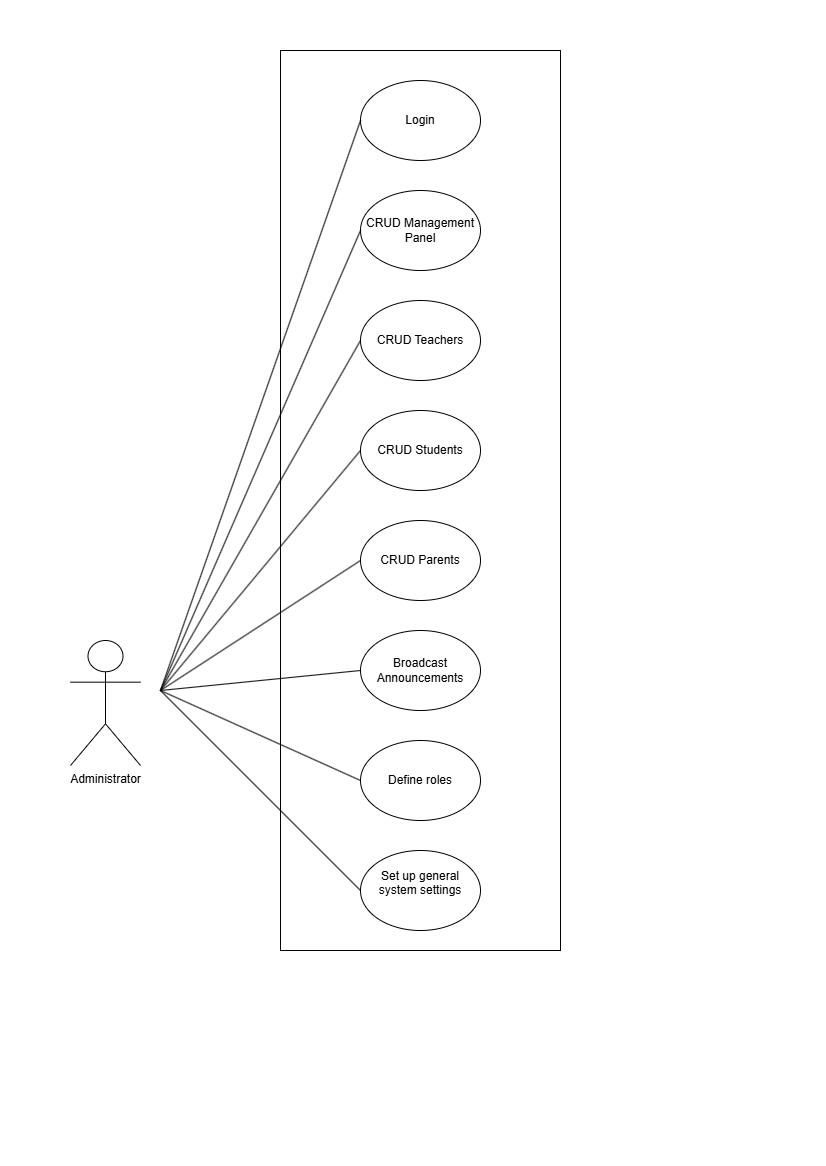
\includegraphics[width=0.8\textwidth,height=0.85\textheight,keepaspectratio]{Diagrams/Use Case/Administrator.png}
    \caption{Administrator Use Case Diagram}
\end{figure}

\begin{figure}[!htbp]
    \centering
    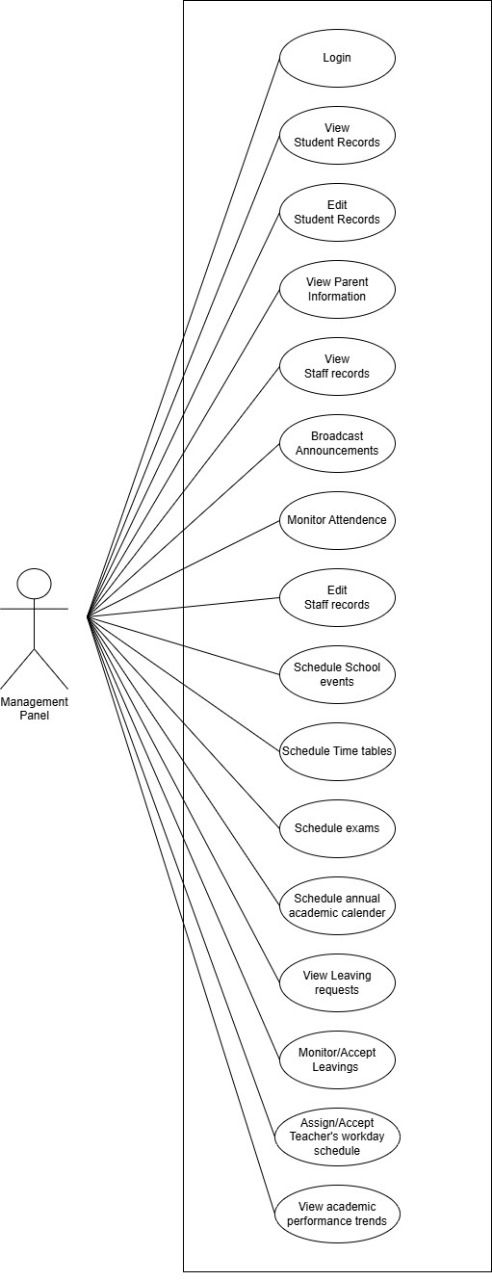
\includegraphics[width=0.8\textwidth,height=0.85\textheight,keepaspectratio]{Diagrams/Use Case/Management Panel.jpg}
    \caption{Management Panel Use Case Diagram}
\end{figure}

\begin{figure}[!htbp]
    \centering
    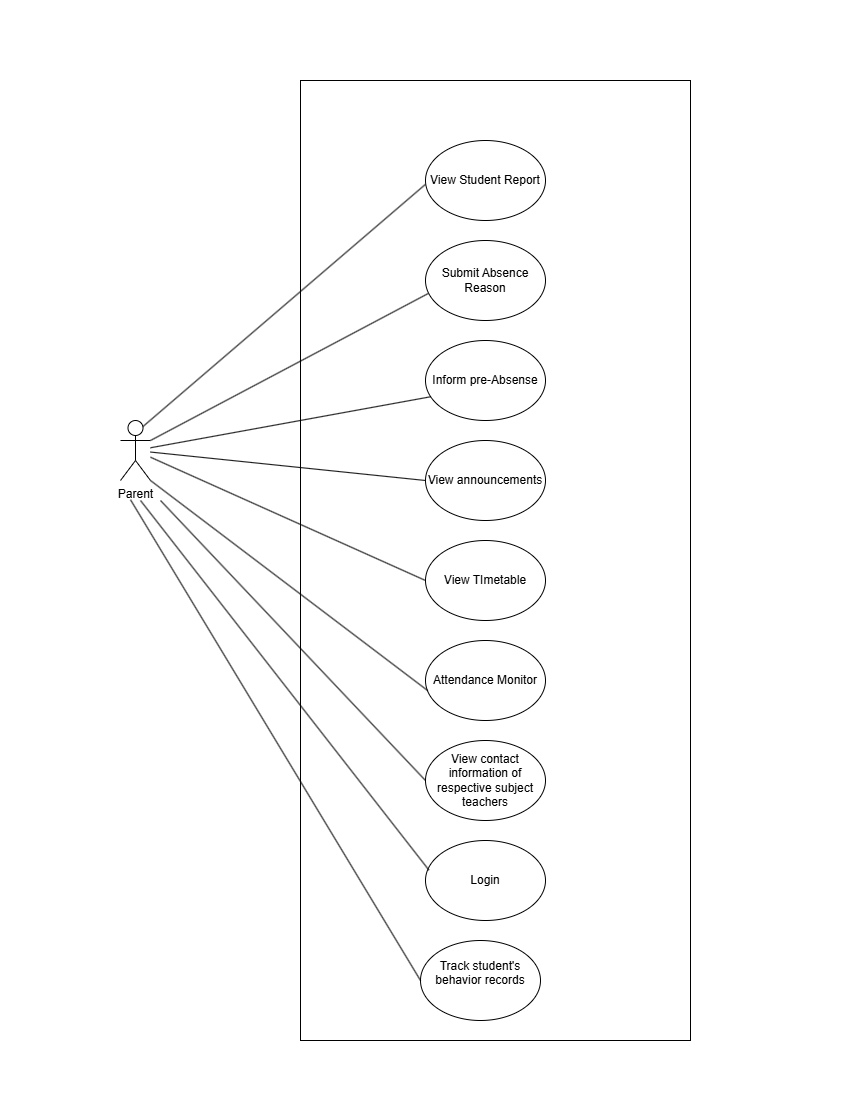
\includegraphics[width=0.8\textwidth,height=0.85\textheight,keepaspectratio]{Diagrams/Use Case/Parent UseCase.png}
    \caption{Parent Use Case Diagram}
\end{figure}

\begin{figure}[!htbp]
    \centering
    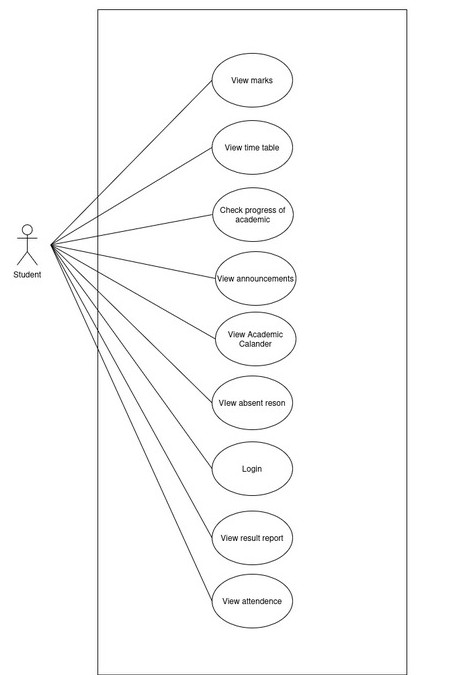
\includegraphics[width=0.8\textwidth,height=0.85\textheight,keepaspectratio]{Diagrams/Use Case/Student.jpg}
    \caption{Student Use Case Diagram}
\end{figure}

\begin{figure}[!htbp]
    \centering
    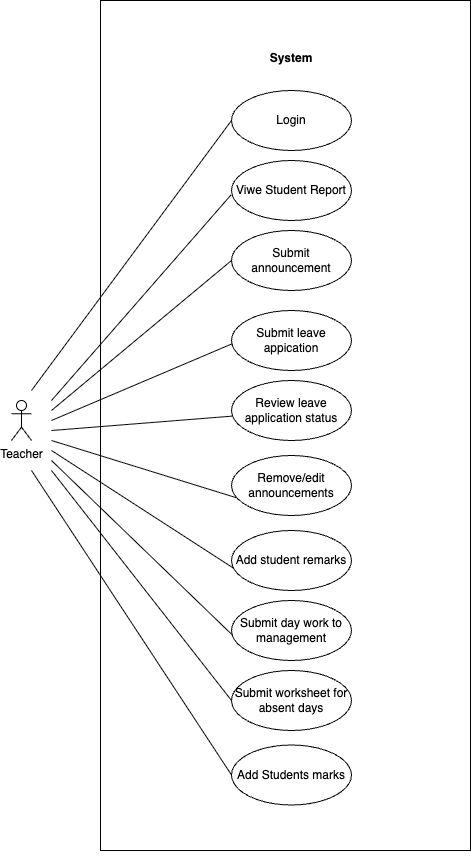
\includegraphics[width=0.8\textwidth,height=0.85\textheight,keepaspectratio]{Diagrams/Use Case/Teacher.jpg}
    \caption{Teacher Use Case Diagram}
\end{figure}

% ── 5.2 ER Diagram ────────────────────────────────────────
\section{ER Diagram}

The Entity-Relationship diagram depicts the database schema, showing all entities, their attributes, and the relationships between them. The system is centred on the \texttt{USER} entity, with specialisations for Student, Teacher, and Parent roles.

\begin{figure}[!htbp]
    \centering
    \includegraphics[width=\textwidth,height=0.85\textheight,keepaspectratio]{Diagrams/ER/iskole_er_diagram.png}
    \caption{ER Diagram}
    \label{fig:er-diagram}
\end{figure}

% ── 5.3 Class Diagram ─────────────────────────────────────
\section{Class Diagram}

The class diagram presents the MVC-based class structure of the system, showing the relationships between Controllers, Models, and Entity classes.

\begin{figure}[!htbp]
    \centering
    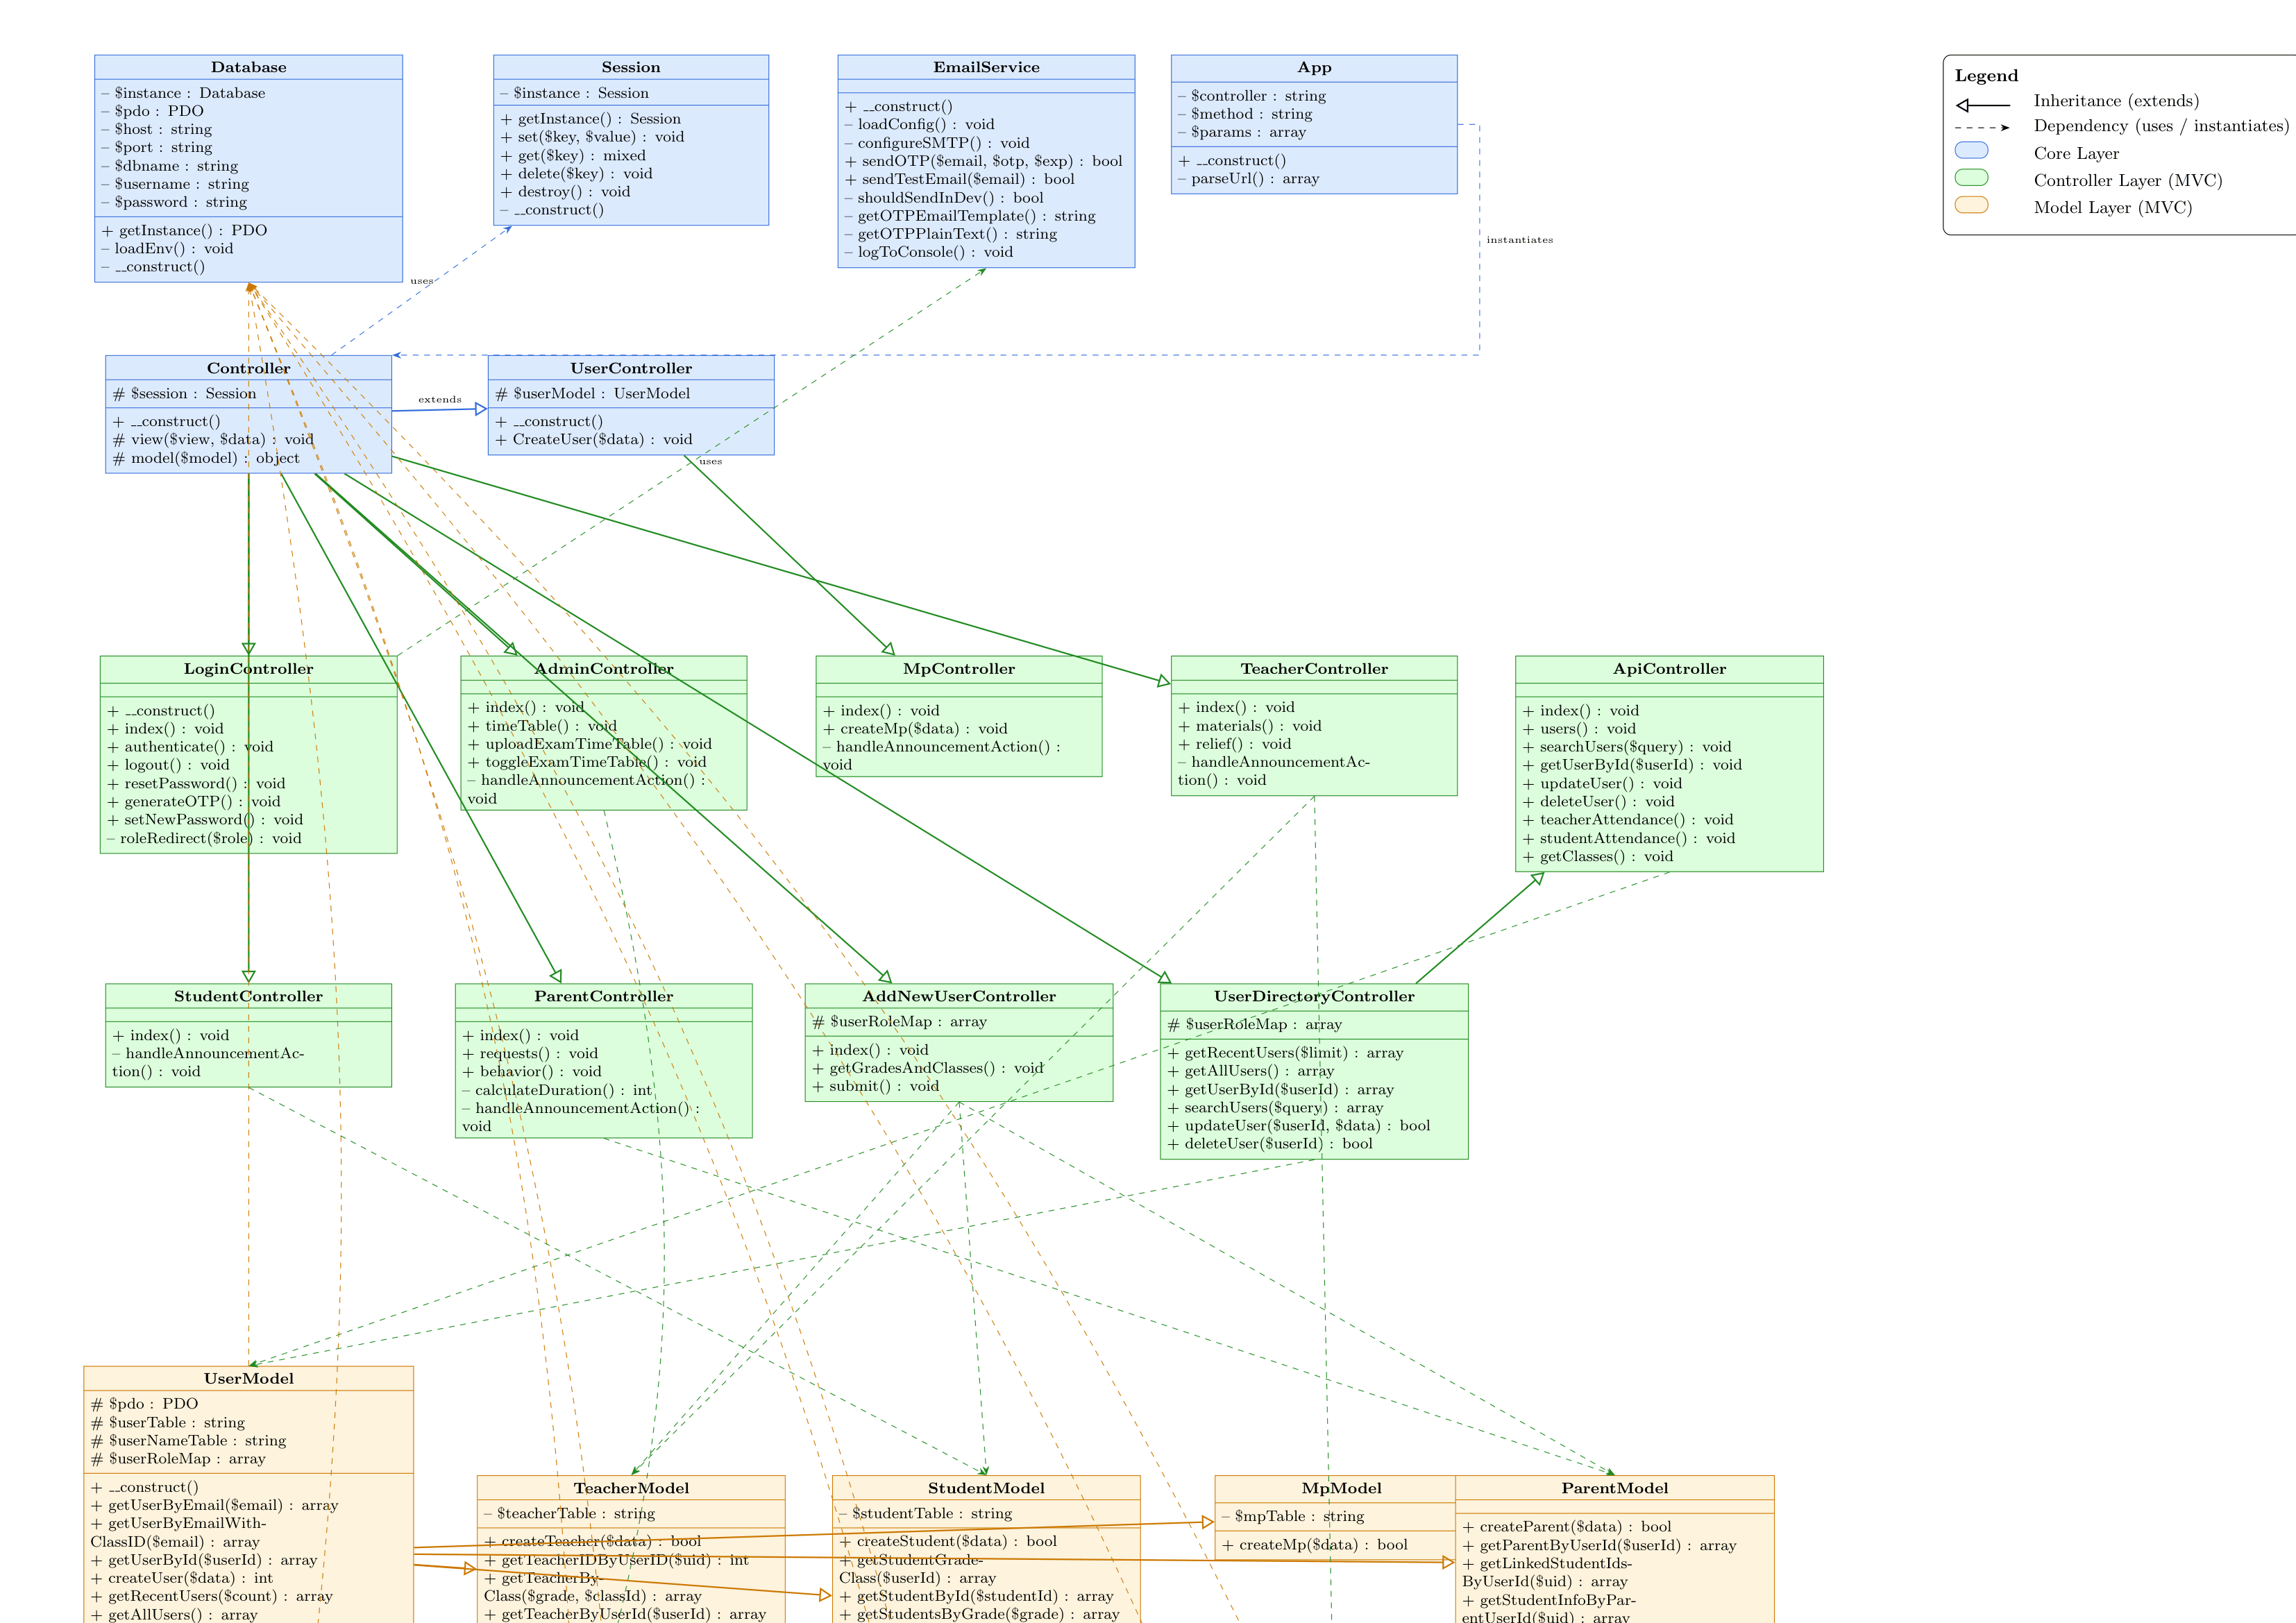
\includegraphics[width=\textwidth,height=0.85\textheight,keepaspectratio]{Diagrams/class_diagram/class_diagram-2.png}
    \caption{Class Diagram}
    \label{fig:class-diagram}
\end{figure}

% ── 5.4 System Architecture Diagram ───────────────────────
\section{System Architecture Diagram}

The system architecture diagram provides a high-level overview of the MVC architecture, illustrating how the front-end, back-end, and database layers interact within the system.

% ── 5.5 Activity Diagrams ─────────────────────────────────
\section{Activity Diagrams}

The activity diagrams depict the flow of operations and interactions for various core functionalities and user roles within the system.

\begin{figure}[!htbp]
    \centering
    
\includegraphics[width=0.8\textwidth,height=0.85\textheight,keepaspectratio]{"Diagrams/Activity/Admin and workflow.png"}
    \caption{Admin Workflow}
\end{figure}

\begin{figure}[!htbp]
    \centering
    
\includegraphics[width=0.8\textwidth,height=0.85\textheight,keepaspectratio]{"Diagrams/Activity/Manager workFlow.png"}
    \caption{Manager Workflow}
\end{figure}

\begin{figure}[!htbp]
    \centering
    
\includegraphics[width=0.8\textwidth,height=0.85\textheight,keepaspectratio]{"Diagrams/Activity/Parent workflow.png"}
    \caption{Parent Workflow}
\end{figure}

\begin{figure}[!htbp]
    \centering
    
\includegraphics[width=0.8\textwidth,height=0.85\textheight,keepaspectratio]{"Diagrams/Activity/Student workflow.png"}
    \caption{Student Workflow}
\end{figure}

\begin{figure}[!htbp]
    \centering
    
\includegraphics[width=0.8\textwidth,height=0.85\textheight,keepaspectratio]{"Diagrams/Activity/Teacher Workflow.png"}
    \caption{Teacher Workflow}
\end{figure}

\begin{figure}[!htbp]
    \centering
    
\includegraphics[width=0.8\textwidth,height=0.85\textheight,keepaspectratio]{"Diagrams/Activity/User Login and password reset.png"}
    \caption{User Login and Password Reset Workflow}
\end{figure}

% ============================================================
%          CHAPTER 6 – COMPLETENESS OF THE PROJECT
% ============================================================
\chapter{Completeness of the Project}

% ── 6.1 Functionalities Completed ─────────────────────────
\section{Functionalities Completed}

All functionalities defined in the project proposal and interim report have been \textbf{100\% completed}. The system consists of \textbf{16 CRUD-based functional modules}, distributed among four group members as follows:

\subsection{R K K Jinendra -- Module Owner}
\begin{enumerate}
    \item Management Staff Records (CRUD)
    \item Teacher Records (CRUD)
    \item Student Records (CRUD)
    \item Parent/Guardian Records (CRUD)
    \item Student Absence Reason Management (CRUD + acknowledgement workflow)
\end{enumerate}

\subsection{Seniru D S Senaweera -- Module Owner}
\begin{enumerate}
    \item Announcements (CRUD)
    \item Learning Materials Management (Upload/Update/Delete/Download)
    \item Teacher Attendance Records (CRUD)
    \item Student Attendance Records (CRUD)
\end{enumerate}

\subsection{S. K. Thasindu Ramsitha -- Module Owner}
\begin{enumerate}
    \item Marks / Exam Results Management (Create/Read/Update)
    \item Student Timetables (CRUD + publish/unpublish)
    \item Teacher Timetables (CRUD + publish/unpublish)
    \item Relief / Teacher Substitution Management (CRUD)
\end{enumerate}

\subsection{R. S. R. G. A. A. Ananda -- Module Owner}
\begin{enumerate}
    \item Classes Management (CRUD)
    \item Exam Timetables (Upload/Update/Delete + image handling)
    \item Teacher Leave Requests (CRUD + approval workflow)
    \item Student Behaviour / Remarks (CRUD)
    \item Subjects Management (CRUD)
\end{enumerate}

% ── 6.2 Functionalities Yet to Complete ───────────────────
\section{Functionalities Yet to Complete}

There are \textbf{no incomplete functionalities}. All planned modules have been successfully implemented and tested.

% ============================================================
%          CHAPTER 7 – INDIVIDUAL CONTRIBUTION ANALYSIS
% ============================================================
\chapter{Individual Contribution Analysis}

All team members contributed equally (25\% each) in the following areas:

\begin{itemize}
    \item System design
    \item Database design
    \item Frontend development
    \item Backend development
    \item Testing
    \item Integration
\end{itemize}

% ── Pie Chart ──────────────────────────────────────────────
\begin{figure}[H]
    \centering
    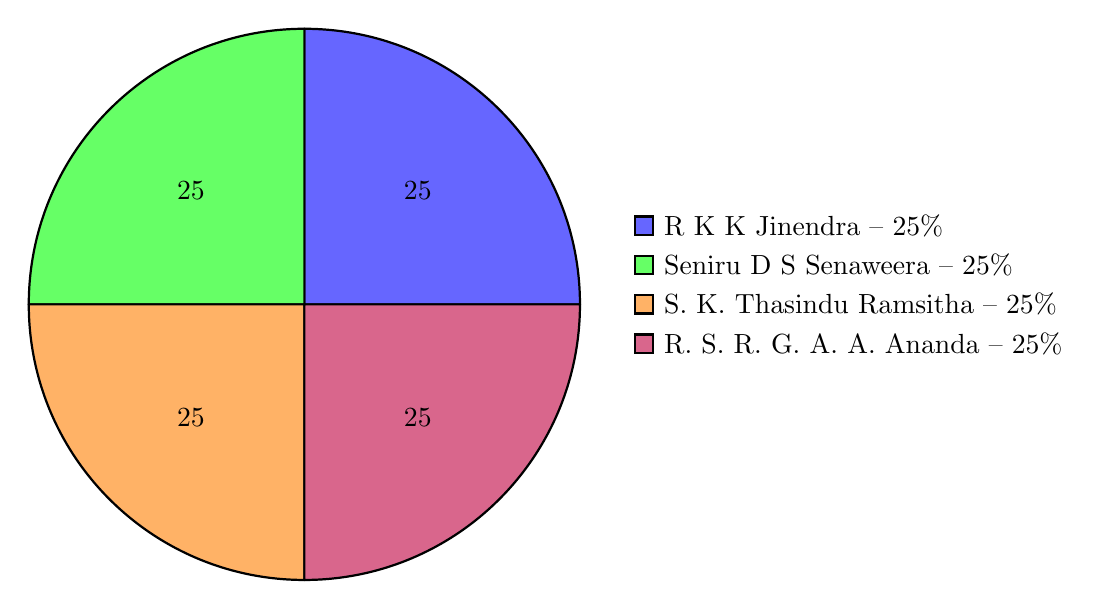
\begin{tikzpicture}
        \pie[
            text=legend,
            radius=3.5,
            color={blue!60, green!60, orange!60, purple!60},
            sum=auto
        ]{
            25/R K K Jinendra -- 25\%,
            25/Seniru D S Senaweera -- 25\%,
            25/S. K. Thasindu Ramsitha -- 25\%,
            25/R. S. R. G. A. A. Ananda -- 25\%
        }
    \end{tikzpicture}
    \caption{Individual Contribution of Team Members}
    \label{fig:contribution-pie}
\end{figure}

\begin{table}[H]
\centering
\caption{Individual Contribution Summary}
\label{tab:contribution}
\begin{tabularx}{\textwidth}{l c >{\raggedright\arraybackslash}X}
\toprule
\textbf{Member} & \textbf{Contribution (\%)} & \textbf{Primary Modules} \\
\midrule
R K K Jinendra  & 25\% & Staff, Teacher, Student, Parent Records; Absence Reasons \\
Seniru D S Senaweera  & 25\% & Announcements, Learning Materials, Attendance Records \\
S. K. Thasindu Ramsitha & 25\% & Marks/Results, Timetables, Relief Management \\
R. S. R. G. A. A. Ananda  & 25\% & Classes, Exam Timetables, Leave Requests, Behaviour, Subjects \\
\bottomrule
\end{tabularx}
\end{table}

% ============================================================
%          CHAPTER 8 – TESTING
% ============================================================
\chapter{Testing}

The system testing was conducted using Google Sheets-based test case documentation. The testing process covered multiple levels to ensure system reliability and correctness.

% ── 8.1 Testing Types ─────────────────────────────────────
\section{Testing Types}

The following testing methodologies were employed:

\begin{enumerate}
    \item \textbf{Unit Testing:} Individual functions and methods within each module were tested in isolation to verify correctness of business logic and data processing.
    \item \textbf{Functional Testing:} End-to-end testing of each functional module to ensure that all features operate as specified in the requirements.
    \item \textbf{CRUD Operation Testing:} Comprehensive testing of all Create, Read, Update, and Delete operations across all 16 functional modules.
    \item \textbf{Integration Testing:} Testing the interactions between interconnected modules to ensure seamless data flow and consistency.
    \item \textbf{Role-Based Access Control Testing:} Verification that each user role (Administrator, Management Panel, Teacher, Student, Parent) has access only to their permitted features and data.
\end{enumerate}

% ── 8.2 Test Case Summary ─────────────────────────────────
\section{Test Case Summary}

\begin{table}[H]
\centering
\caption{Testing Summary}
\label{tab:testing-summary}
\begin{tabular}{l l}
\toprule
\textbf{Aspect} & \textbf{Details} \\
\midrule
Total Functional Units        & 16 modules \\
Testing Approach              & Module-level and integration testing \\
CRUD Operations               & All operations validated for correctness \\
Role-Based Access Control     & Verified for all 5 user roles \\
Test Documentation            & Google Sheets-based test case tracking \\
Test Result                   & All test cases passed successfully \\
\bottomrule
\end{tabular}
\end{table}

\noindent\textit{Note: The complete Google Sheets test case document is available at \url{https://docs.google.com/spreadsheets/d/14EDXcn4uQs7-RyXaZ515DG7CmKuiKECqpi0Rp3X_nPk/edit?usp=sharing}.}

% ============================================================
%          CHAPTER 9 – SUPERVISOR DETAILS
% ============================================================
\chapter{Details of Project Supervisor and Co-Supervisor}

\section*{Proposed Project Supervisor (Academic Staff of UCSC)}

\noindent
\begin{tabular}{@{} p{6cm} p{8cm} @{}}
Name of the supervisor: & Mr.\ Viraj Welgama \\[1cm]
Signature of the supervisor: & \rule{6cm}{0.4pt} \\[1cm]
Date: & \rule{6cm}{0.4pt} \\
\end{tabular}

\vspace{1cm}

\section*{Proposed Project Co-Supervisor (Assigned by the Course Coordinator)}

\noindent
\begin{tabular}{@{} p{6cm} p{8cm} @{}}
Name of the co-supervisor: & Mr.\ Janitha Dissanayake \\[1cm]
Signature of the co-supervisor: & \rule{6cm}{0.4pt} \\[1cm]
Date: & \rule{6cm}{0.4pt} \\
\end{tabular}

% ============================================================
%          CHAPTER 10 – DECLARATION
% ============================================================
\chapter{Declaration}

We, as members of the project titled \textbf{IskolE}, certify that we will carry out this project according to the guidelines provided by the coordinators and supervisors of the course, as well as that we will not incorporate, without acknowledgment, any material previously submitted for a degree or diploma in any university.

To the best of our knowledge and belief, the project work will not contain any material previously published or written by another person or ourselves except where due reference is made in the text at appropriate places.

\vspace{2cm}

\begin{figure}[!htbp]
    \centering
    \includegraphics[width=\textwidth,height=0.85\textheight,keepaspectratio]{"members.png"}
\end{figure}

% ============================================================
\end{document}
